\documentclass[UTF8]{beamer}

\usepackage{minted}
\newminted{c}{autogobble,breaklines,linenos,mathescape}

\usepackage{xeCJK}
\setCJKmainfont{STFangsong}
\usetheme{CambridgeUS}

\AtBeginSection[]
{
  \begin{frame}<beamer>{目录}
    \tableofcontents[
      currentsection,
      currentsubsection,
      hideothersubsections,
      sectionstyle=show/shaded,
    ]
  \end{frame}
}
\setbeamerfont{subsection in toc}{size=\small}
\setbeamersize{text margin left=2em}

\title{Unix Socket 编程入门}
\author{吕海涛 \\ \texttt{share@lvht.net}}
\date{\today}

\begin{document}
\begin{frame}
  \titlepage
\end{frame}
\section{基本概念}
\subsection{字节顺序}
\begin{frame}{大端与小端}
  \centerline{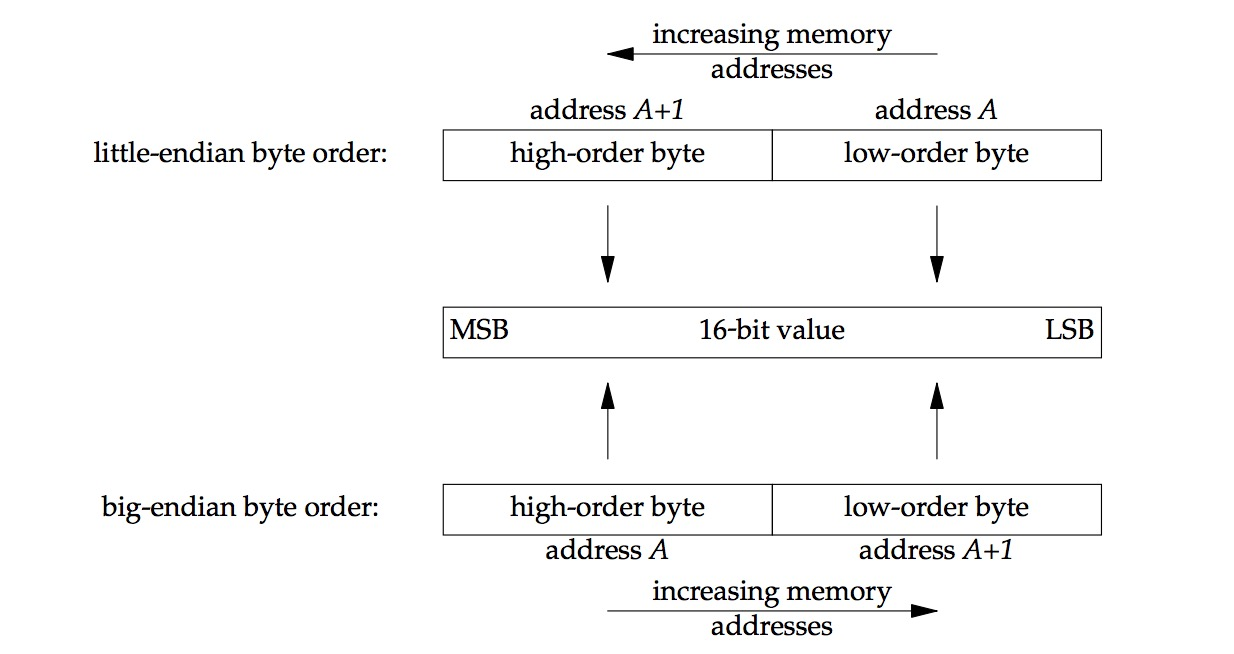
\includegraphics[width=\textwidth]{img/byte-order.png}}
\end{frame}
\begin{frame}[fragile]{检查字节顺序}
  \begin{ccode}
    #include <arpa/inet.h>

    union { int16_t s; char c[2]; } un;

    un.s = 0x0102;
    printf("host:0x0102 => %d-%d\n", un.c[0], un.c[1]);
    un.s = htons(0x0102);
    printf("net:0x0102 => %d-%d\n", un.c[0], un.c[1]);
  \end{ccode}
\end{frame}
\begin{frame}[fragile]{字节顺序转换}
  网络数据传输使用\textbf{大端}字节顺序!
  \begin{ccode}
     #include <arpa/inet.h>

     uint32_t htonl(uint32_t hostlong);
     uint16_t htons(uint16_t hostshort);
     uint32_t ntohl(uint32_t netlong);
     uint16_t ntohs(uint16_t netshort);
  \end{ccode}
\end{frame}
\subsection{IP地址表示}
\begin{frame}[fragile]{IP地址结构体}
  \begin{ccode}
    #include <netinet/in.h>

    struct sockaddr_in {
      short          sin_family;  // e.g. AF_INET
      unsigned short sin_port;    // e.g. htons(3490)
      struct in_addr sin_addr;    // see struct in_addr, below
      char           sin_zero[8]; // zero this if you want to
    };

    struct in_addr {
      unsigned long s_addr;  // load with inet_aton()
    };
  \end{ccode}
\end{frame}
\begin{frame}[fragile]{IP地址转换}
  \begin{ccode}
    #include <arpa/inet.h>

    int inet_aton(const char *strptr, struct in_addr *addrptr);
    char *inet_ntoa(struct in_addr inaddr);

    int inet_pton(int family, const char *strptr, void *addrptr);
    const char *inet_ntop(int family, const void *addrptr, char *strptr, size_t len);
  \end{ccode}
\end{frame}
\subsection{TCP/IP通信流程}
\begin{frame}{TCP/IP通信流程}
  \centerline{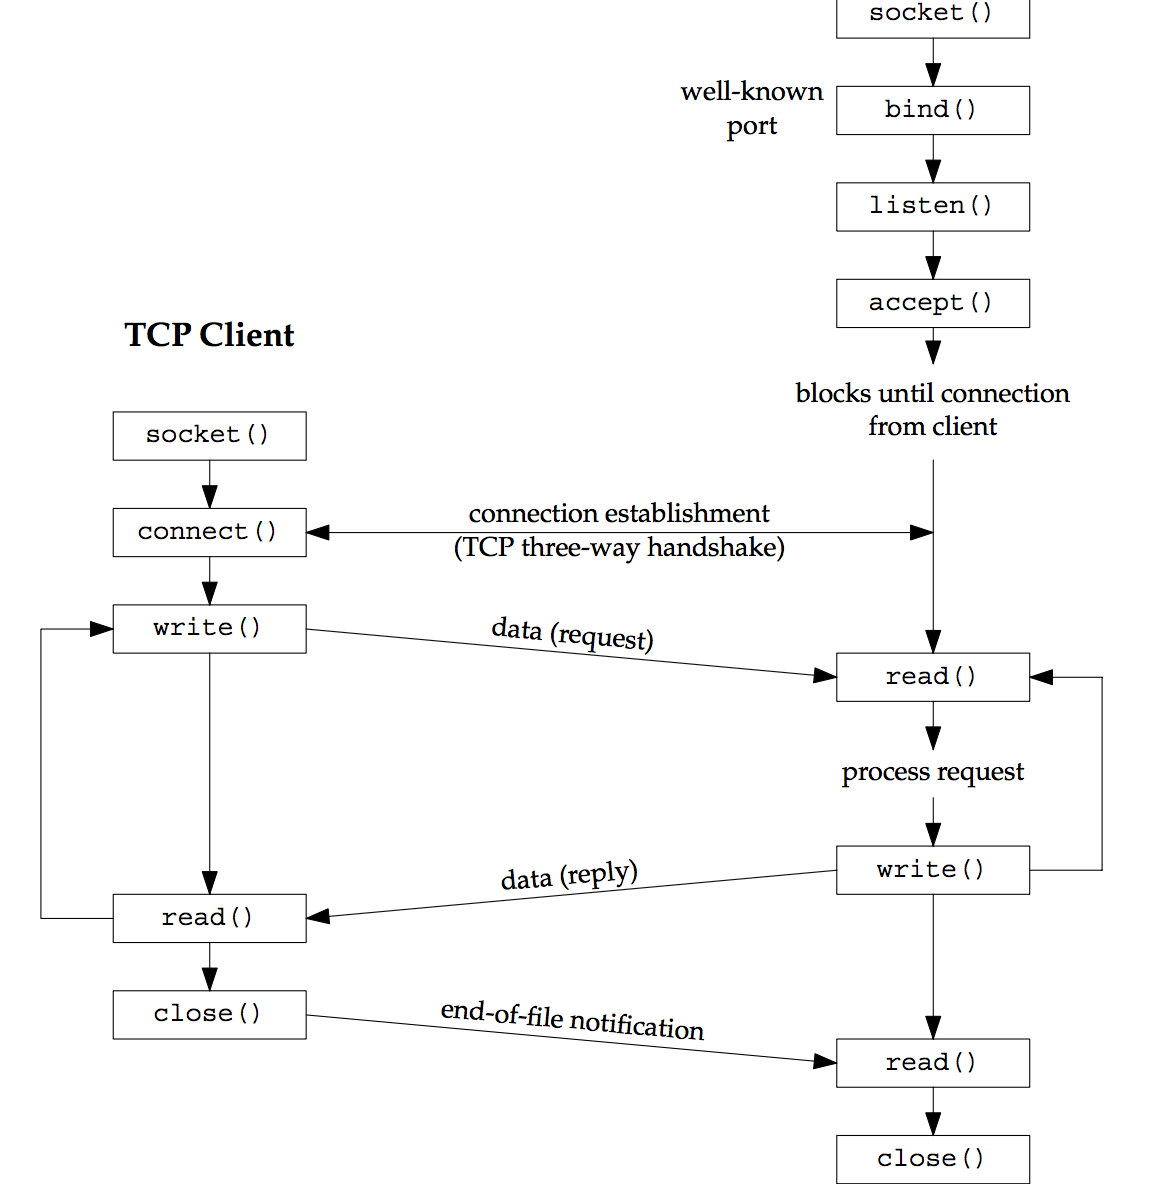
\includegraphics[height=\textheight]{img/tcp.png}}
\end{frame}
\section{网络系统调用}
\subsection{系统调用列表}
\begin{frame}[fragile]
  \begin{ccode}
    #include <sys/socket.h>

    int socket(int family, int type, int protocol);
    int connect(int sockfd, const struct sockaddr *servaddr, socklen_t addrlen);
    int bind(int sockfd, const struct sockaddr *myaddr, socklen_t addrlen);
    int listen(int sockfd, int backlog);
    int accept(int sockfd, struct sockaddr *cliaddr, socklen_t *addrlen);
    int send(int socket, const void *buffer, int length, int flags);
    int recv(int socket, void *buffer, int length, int flags);
    int close(int sockfd);
  \end{ccode}
\end{frame}
\subsection{socket()}
\begin{frame}[fragile]{socket}
  \begin{ccode}
    int socket(int family, int type, int protocol);
  \end{ccode}
  \pause
  \begin{columns}
    \only<1> {
      \begin{column}{\textwidth}
        \begin{center}
          \begin{tabular}{ | l | c | r }
            \hline
            family & Description \\ \hline
            AF\_INET & IPv4 protocols \\
            AF\_INET6 & IPv6 protocols \\
            AF\_LOCAL & Unix domain protocols \\
            \hline
          \end{tabular}
        \end{center}
      \end{column}
    }
    \only<2> {
      \begin{column}{\textwidth}
        \begin{center}
          \begin{tabular}{ | l | c | r }
            \hline
            type & Description \\ \hline
            SOCK\_STREAM & stream socket \\
            SOCKAF\_DGRAM & datagram socket \\
            \hline
          \end{tabular}
        \end{center}
      \end{column}
    }
    \only<3> {
      \begin{column}{\textwidth}
        \begin{center}
          \begin{tabular}{ | l | c | r }
            \hline
            protocol & Description \\ \hline
            IPPROTO\_TCP & TCP transport protocol \\
            IPPROTO\_UDP & TCP transport protocol \\
            IPPROTO\_SCTP & TCP transport protocol \\
            \hline
          \end{tabular}
        \end{center}
      \end{column}
    }
  \end{columns}
\end{frame}
\subsection{listen()}
\begin{frame}[fragile]{listen}
  \begin{ccode}
    int listen(int sockfd, int backlog);
  \end{ccode}
  \begin{columns}
    \pause
    \begin{column}{0.5\textwidth}
      \begin{center}
        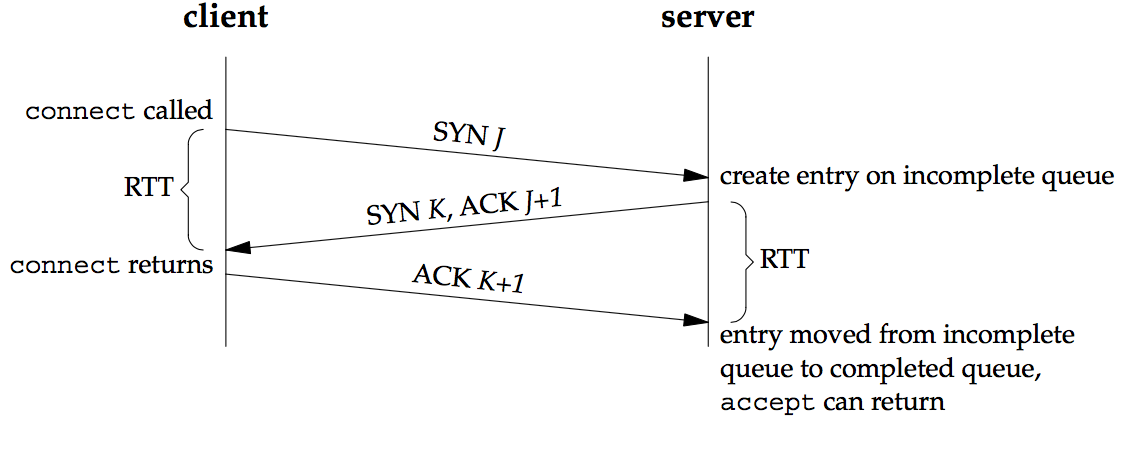
\includegraphics[width=\textwidth]{img/3-way-handshake.png}
      \end{center}
    \end{column}
    \pause
    \begin{column}{0.5\textwidth}
      \begin{center}
        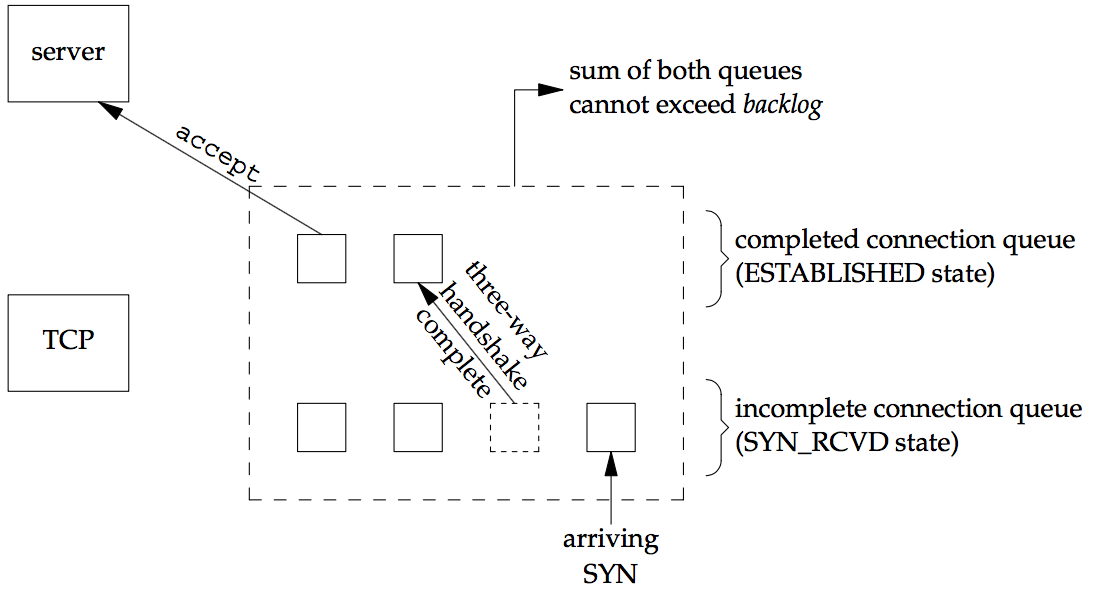
\includegraphics[width=\textwidth]{img/backlog.png}
      \end{center}
    \end{column}
  \end{columns}
\end{frame}
\section{示例代码}
\subsection{客户端示例}
\begin{frame}[fragile]{获取服务端IP}
  \begin{ccode}
    int sockfd, numbytes, rv;
    char ip[INET6_ADDRSTRLEN];
    char buf[1024];
    struct addrinfo hints, *servinfo, *p;
    memset(&hints, 0, sizeof hints);
    hints.ai_family = AF_UNSPEC;
    hints.ai_socktype = SOCK_STREAM;

    if ((rv = getaddrinfo("bilibili.com", "http", &hints, &servinfo)) != 0) {
      fprintf(stderr, "getaddrinfo: %s\n", gai_strerror(rv));
      return 1;
    }
  \end{ccode}
\end{frame}
\begin{frame}[fragile]{发起TCP连接}
  \begin{ccode}
    for (p = servinfo; p != NULL; p = p->ai_next) {
      if ((sockfd = socket(p->ai_family, p->ai_socktype, p->ai_protocol)) == -1) {
        perror("==> client: socket");
        continue;
      }
      if (connect(sockfd, p->ai_addr, p->ai_addrlen) == -1) {
        perror("==> client: connect");
        continue;
      }
      break;
    }
  \end{ccode}
\end{frame}
\begin{frame}[fragile]{收发HTTP数据}
  \begin{ccode}
    char req[] = "GET / HTTP/1.0\r\nHost: bilibili.com\r\n\r\n";
    if ((numbytes = recv(sockfd, buf, 1024, 0)) == -1) {
      perror("==> client: recv");
      return 3;
    }
    if ((numbytes = recv(sockfd, buf, 1024, 0)) == -1) {
      perror("==> client: recv");
      return 3;
    }
    printf("==> client: received\n%.*s", numbytes, buf);

    close(sockfd);
  \end{ccode}
\end{frame}
\subsection{服务端示例}
\begin{frame}[fragile]{数据初始化}
  \begin{ccode}
    int listen_fd, conn_fd, recv_num;
    struct sockaddr_in serv_addr, cli_addr;
    char buf[1024];

    listen_fd = socket(PF_INET, SOCK_STREAM, IPPROTO_TCP);
    if (listen_fd == -1) {
      perror("==> server: socket");
      return 1;
    }

    memset(&serv_addr, 0, sizeof serv_addr);
    serv_addr.sin_family = AF_INET;
    serv_addr.sin_addr.s_addr = htonl(INADDR_ANY);
    serv_addr.sin_port = htons(1234);
  \end{ccode}
\end{frame}
\begin{frame}[fragile]{监听端口}
  \begin{ccode}
    if (bind(listen_fd, (struct sockaddr *)&serv_addr, sizeof serv_addr) == -1) {
      perror("==> server: bind");
      return 2;
    }

    if (listen(listen_fd, 1) == -1) {
      perror("==> server: listen");
      return 3;
    }
  \end{ccode}
\end{frame}
\begin{frame}[fragile]{处理连接}
  \begin{ccode}
    while (1) {
      int cli_addr_len = sizeof cli_addr;
      conn_fd = accept(listen_fd, (struct sockaddr *)&cli_addr, &cli_addr_len);
      if (conn_fd == -1) {
        perror("==> server: accept");
        continue;
      }
      do {
        recv_num = recv(conn_fd, buf, sizeof buf, 0);
        send(conn_fd, buf, recv_num, 0);
      } while (recv_num > 0);
      close(conn_fd);
    }
  \end{ccode}
\end{frame}
\section{IO模型}
\subsection{阻塞IO}
\begin{frame}{阻塞IO}
  \centerline{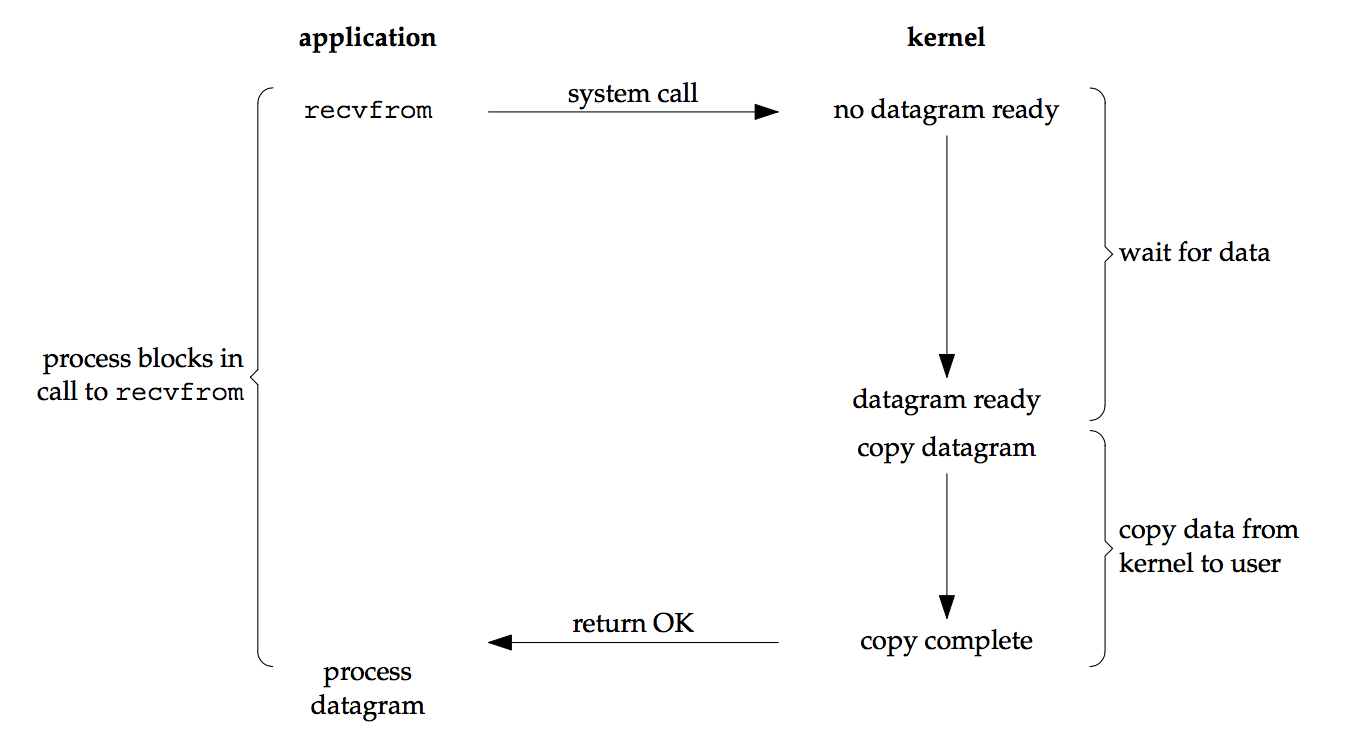
\includegraphics[width=\textwidth]{img/block.png}}
\end{frame}
\subsection{非阻塞IO}
\begin{frame}{非阻塞IO}
  \centerline{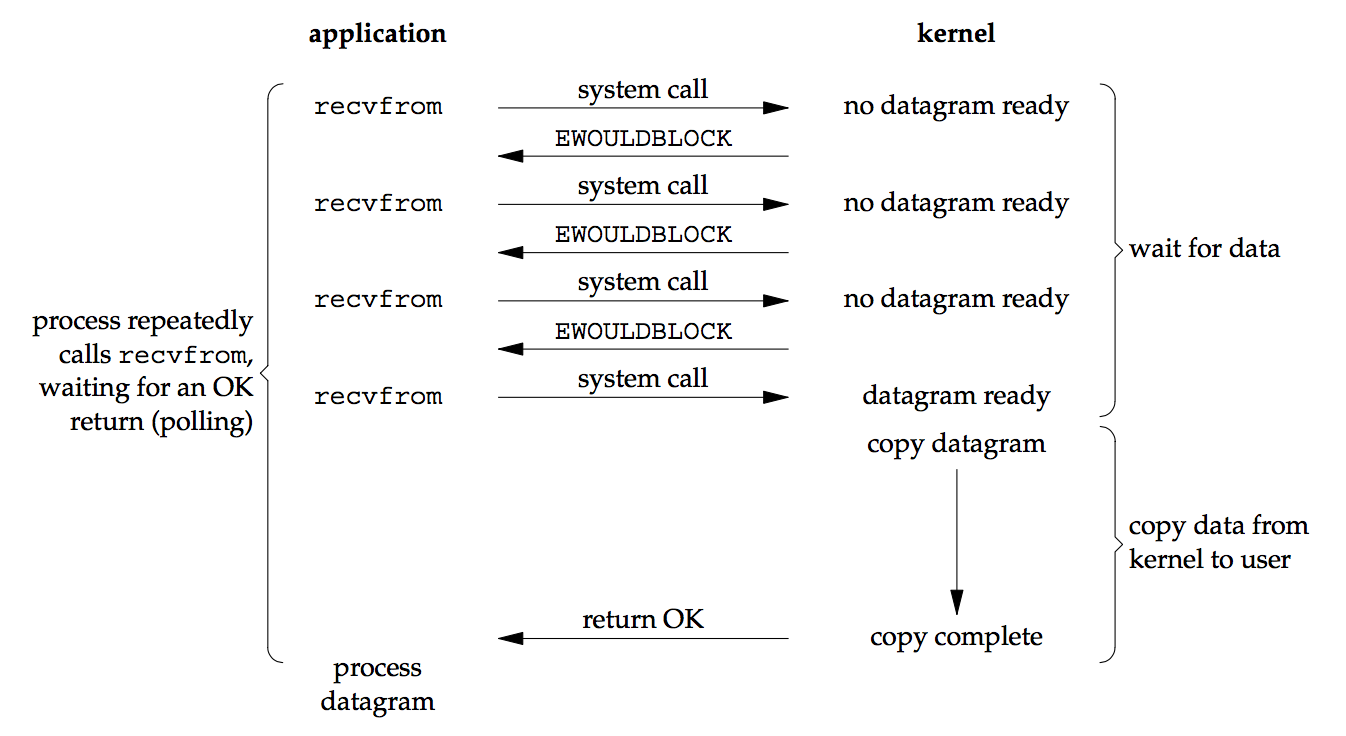
\includegraphics[width=\textwidth]{img/non-block.png}}
\end{frame}
\section{IO多路复用}
\begin{frame}{总体流程}
  \centerline{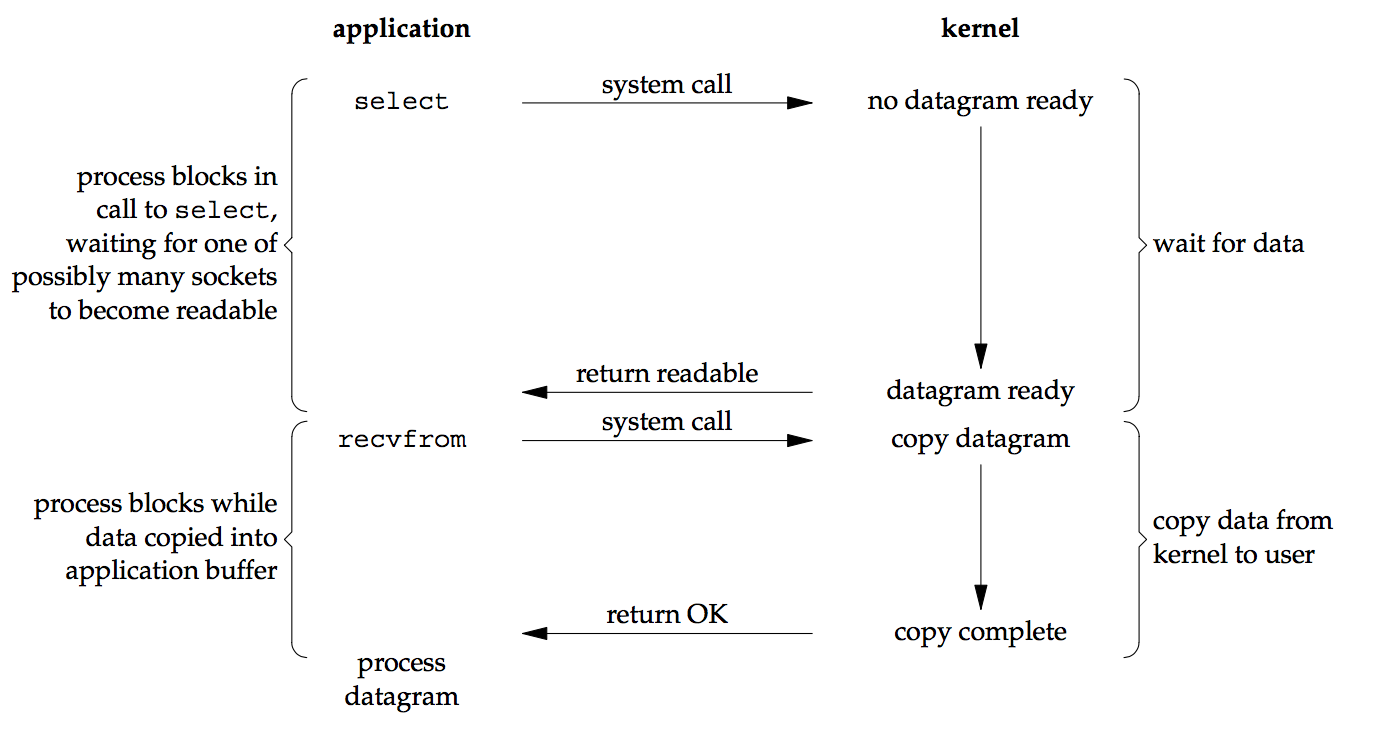
\includegraphics[width=\textwidth]{img/multi-io.png}}
\end{frame}
\subsection{select}
\begin{frame}[fragile]{select系统调用}
  \begin{ccode}
    #include <sys/select.h>
    #include <sys/time.h>
    int select(int maxfdp1, fd_set *readset, fd_set *writeset, fd_set *exceptset, const struct timeval *timeout);

    /* clear all bits in fdset */
    void FD_ZERO(fd_set *fdset);
    /* turn on the bit for fd in fdset */
    void FD_SET(int fd, fd_set *fdset);
    /* turn off the bit for fd in fdset */
    void FD_CLR(int fd, fd_set *fdset);
    /* is the bit for fd on in fdset ? */
    int FD_ISSET(int fd, fd_set *fdset);

    struct timeval { long tv_sec; long tv_usec; };
  \end{ccode}
\end{frame}
\begin{frame}[fragile]{初始化}
  \begin{ccode}
    // ...
    fd_set fds, fds2;
    int fdmax;
    fcntl(listen_fd, F_SETFL, O_NONBLOCK);

    FD_ZERO(&fds);
    FD_SET(listen_fd, &fds);
    fdmax = listen_fd;
  \end{ccode}
\end{frame}
\begin{frame}[fragile]{主事件循环}
  \begin{ccode}
    while (1) {
      fds2 = fds; // why?
      if (select(fdmax+1, &fds2, NULL, NULL, NULL) == -1) {
        perror("==> server: select");
        return 4;
      }
      // check every fd
    }
  \end{ccode}
\end{frame}
\begin{frame}[fragile]{fd事件检查}
  \begin{ccode}
    for (int i = 0; i <= fdmax; i++) {
      if (!FD_ISSET(i, &fds2)) continue;
      if (i == listen_fd) { // listen socket has new connection
        int cli_addr_len = sizeof cli_addr;
        conn_fd = accept(listen_fd, (struct sockaddr *)&cli_addr, &cli_addr_len);
        fcntl(conn_fd, F_SETFL, O_NONBLOCK);
        FD_SET(conn_fd, &fds);
        if (conn_fd > fdmax) fdmax = conn_fd;
      } else { // client sent data to us
        recv_num = recv(i, buf, sizeof buf, 0);
        if (recv_num > 0) { send(i, buf, recv_num, 0); }
        else {
          FD_CLR(i, &fds); close(i);
        }
      }
    }
  \end{ccode}
\end{frame}
\begin{frame}[fragile]{select不足}
  \begin{enumerate}
      \item 每次调用select函数后需要重复设置fd\_set
      \item select函数返回后需要遍历所有fd $O(n)$
      \item fd\_set 容量有限 $<1024$
  \end{enumerate}
\end{frame}
\subsection{poll}
\begin{frame}[fragile]{poll系统调用}
  \begin{ccode}
    #include <poll.h>
    int poll(struct pollfd *fdarray, unsigned long nfds, int timeout);

    struct pollfd {
      int    fd;       /* descriptor to check */
      short  events;   /* events of interest on fd */
      short  revents;  /* events that occurred on fd */
    };
  \end{ccode}
\end{frame}
\begin{frame}[fragile]{初始化}
  \begin{ccode}
    struct poolfd fds[1024];
    int fdmax, nready;
    fds[0].fd = listen_fd;
    fds[0].events = POLLRDNORM; // monitor read
    fdmax = 0;
    for (int i = 1; i < 1024; i++) {
      fds[i].fd = -1;
    }
  \end{ccode}
\end{frame}
\begin{frame}[fragile]{主事件循环}
  \begin{ccode}
    while (1) {
      if (nready = pool(fds, fdmax + 1, NULL, INFTIM) == -1) {
        perror("==> server: pool");
        return 4;
      }
      // check fd
    }
  \end{ccode}
\end{frame}
\begin{frame}[fragile]{检查传入连接}
  \begin{ccode}
    if (fds[0].revents & POLLRDNORM) {
      int cli_addr_len = sizeof cli_addr;
      conn_fd = accept(listen_fd, (struct sockaddr *)&cli_addr, &cli_addr_len);
      fcntl(conn_fd, F_SETFL, O_NONBLOCK);
      if (conn_fd > fdmax) fdmax = conn_fd;
      for (int i = 0; i < 1024; i++) {
        if (fds[i].fd < 0) {
          fds[i].fd = conn_fd;
          fds[i].events = POLLRDNORM;
          break;
        }
      }
      // error check
      if (--nready <= 0) continue;
    }
  \end{ccode}
\end{frame}
\begin{frame}[fragile]{接收客户端数据}
  \begin{ccode}
    for (int i = 1; i <= fdmax; i++) {
      int fd = fds[i].fd;
      if (fd < 0) continue;
      if (fds[i].revents & POLLRDNORM) {
        recv_num = recv(fd, buf, sizeof buf, 0);
        if (recv_num > 0) {
          send(fd, buf, recv_num, 0);
        } else {
          fds[i].fd = -1;
          close(i);
        }
      }
    }
  \end{ccode}
\end{frame}
\begin{frame}[fragile]{poll不足}
  \begin{enumerate}
    \item \mintinline{c}{struct pollfd} 不够灵活
    \item pool函数返回后需要遍历所有fd $O(n)$
  \end{enumerate}
\end{frame}
\subsection{kqueue}
\begin{frame}[fragile]{kqueue系统调用}
  \begin{ccode}
  \end{ccode}
\end{frame}
\begin{frame}[fragile]{kqueue流程}
  \begin{ccode}
  \end{ccode}
\end{frame}
\begin{frame}[fragile]{kqueue不足}
  \begin{ccode}
  \end{ccode}
\end{frame}
\section{主要服务端软件IO模型}
\subsection{php-fpm}
\begin{frame}[fragile]{php-fpm}
  \begin{ccode}
  \end{ccode}
\end{frame}
\subsection{memcached}
\begin{frame}[fragile]{memcached}
  \begin{ccode}
  \end{ccode}
\end{frame}
\subsection{nginx}
\begin{frame}[fragile]{nginx}
  \begin{ccode}
  \end{ccode}
\end{frame}
\subsection{swoole}
\begin{frame}[fragile]{swoole}
  \begin{ccode}
  \end{ccode}
\end{frame}
\end{document}
